\documentclass[11pt]{article}
\usepackage[spanish]{babel}
\usepackage[utf8]{inputenc}
\usepackage{listings}
\usepackage{graphicx}
\graphicspath{{../Imagenes/}}

\usepackage[paper=portrait, pagesize]{typearea}
\usepackage{titlepic}

%%% Tablas
\usepackage{tabularx}
\usepackage{float}
\usepackage{adjustbox}
\usepackage{booktabs}
\usepackage{multirow}
\renewcommand{\arraystretch}{1.7}

\begin{document}

\begin{titlepage}
\centering
\vspace{4.5cm}
{\scshape\LARGE Descripción de personajes y escenarios\par}
{\scshape\LARGE Peña de Fútbol\par}
\vspace{1.5cm}

{\scshape\large \today \par}
\vspace{14cm}

{Miguel Albertí Pons\\
Sofía Almeida Bruno\\
Pedro Manuel Flores Crespo\\
María Victoria Granados Pozo\\
Lidia Martín Chica
\par}

\end{titlepage}


\newpage

\section{Personajes}
%%TABLA MANUEL
\begin{table}[H]
  \centering
  \begin{tabular}{p{0.2\linewidth}|p{0.3\linewidth}p{0.475\linewidth}}
    \toprule
    \textbf{Nombre} & Manuel Navarro Vázquez &\multirow{4}{*}{FOTO}\\
    \textbf{Edad} & 43 & \\
    \textbf{Sexo} & Hombre & \\
    \textbf{Educación} & Trabaja de policía & \\
    \bottomrule
  \end{tabular}

  \begin{tabular}{l}
    \textbf{Contexto de uso} 
  \end{tabular}
  
  \begin{tabular}{p{0.2\linewidth}|p{0.8\linewidth}}
    \toprule
    \textbf{Cuándo} & Por las mañanas antes de empezar a trabajar\\
    \textbf{Dónde}  & En su casa\\
    \textbf{Tipo de ordenador} & Tiene un móvil no muy moderno\\
    \bottomrule
  \end{tabular}

  \begin{tabular}{l}
    \textbf{Misión} 
  \end{tabular}
  
  \begin{tabular}{p{0.2\linewidth}|p{0.8\linewidth}}
    \toprule
    \textbf{Objetivo} & Subir noticias sobre los equipos a diario, además de informar sobre la organización de los viajes\\
    \textbf{Expectativas}  & Facilidad a la hora de actualizar contenido. Distintas secciones: una para noticias y otra para viajes \\
    \bottomrule
  \end{tabular}

  \begin{tabular}{l}
    \textbf{Motivación} 
  \end{tabular}

  \begin{tabular}{p{0.2\linewidth}|p{0.8\linewidth}}
    \toprule
    \textbf{Urgencia} & Alta, debe poder actualizar la información a diario\\
    \textbf{Deseo}  & Mantener a los aficionados que utilicen la aplicación al día sobre las novedades en este deporte, especialmente las que refieran al Granada. Organizar los viajes de la peña.\\
    \bottomrule
  \end{tabular}

  \begin{tabular}{p{1.028\linewidth}}
    \textbf{Actitud hacia la tecnología}\\
    \midrule
    Utiliza el móvil con facilidad, especialmente las aplicaciones que ya conoce. 
  \end{tabular}
\end{table}

%%TABLA ELENA
\begin{table}[H]
  \centering
  \begin{tabular}{p{0.2\linewidth}|p{0.3\linewidth}p{0.475\linewidth}}
    \toprule
    \textbf{Nombre} & Elena Luzón Pérez  &\\\multirow{4}{*}{\begin{minipage}{1.\textwidth}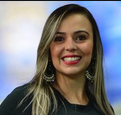
\includegraphics[width=0.2\textwidth, height=30mm]{Elena}\end{minipage}}\\
    \textbf{Edad} & 29 & \\
    \textbf{Sexo} & Mujer & \\
    \textbf{Educación} & Graduada en educación primaria & \\
    \bottomrule
  \end{tabular}

  \begin{tabular}{l}
    \textbf{Contexto de uso} 
  \end{tabular}
  
  \begin{tabular}{p{0.2\linewidth}|p{0.8\linewidth}}
    \toprule
    \textbf{Cuándo} & El domingo, ya que es su día libre en la preparación de las oposiciones\\
    \textbf{Dónde}  & En su casa\\
    \textbf{Tipo de ordenador} & En este caso, utiliza su dispositivo móvil\\
    \bottomrule
  \end{tabular}

  \begin{tabular}{l}
    \textbf{Misión} 
  \end{tabular}
  
  \begin{tabular}{p{0.2\linewidth}|p{0.8\linewidth}}
    \toprule
    \textbf{Objetivo} & Organizar un viaje a Turquía\\
    \textbf{Expectativas}  & Estar al día de los resultados de los partidos del equipo y de las noticias \\
    \bottomrule
  \end{tabular}

  \begin{tabular}{l}
    \textbf{Motivación} 
  \end{tabular}

  \begin{tabular}{p{0.2\linewidth}|p{0.8\linewidth}}
    \toprule
    \textbf{Urgencia} & Mínima, cuando tenga interés abrirá la aplicación\\
    \textbf{Deseo}  & Estar informada acerca del equipo de fútbol granadino \\
    \bottomrule
  \end{tabular}

  \begin{tabular}{p{1.028\linewidth}}
    \textbf{Actitud hacia la tecnología}\\
    \midrule
    Se maneja con el móvil y la tablet a nivel de usuario
  \end{tabular}
\end{table}

\end{document}
